\documentclass[twocolumn,twoside,a4paper,10pt]{IEEEtran}

\usepackage[utf8]{inputenc}
\usepackage[T1]{fontenc}
\usepackage[noadjust]{cite}
    \renewcommand{\citepunct}{,\penalty\citepunctpenalty\,}
    \renewcommand{\citedash}{--}
\usepackage{url}
\usepackage{graphicx}
\usepackage{xcolor}
\usepackage{hyperref}
    \hypersetup{
        colorlinks,
        linkcolor={red!50!black},
        citecolor={blue!50!black},
        urlcolor={blue!80!black}
    }
\usepackage{amsmath}
\usepackage{booktabs}

% The first path is used when compiling from thesis/; the second also permits
% compilation from the repository root.
\graphicspath{{../results/figures/eda/}{../results/metrics/}
              {results/figures/eda/}{results/metrics/}}

% Spanish and Catalan are defined because titlepage.tex tests both languages;
% English remains the active language because it is listed last.
\usepackage[spanish,catalan,english]{babel}
\title{Hydrological Modelling of the Sant Miquel Basin: A Comparative Study of Physics-Based and Machine Learning Approaches}
\author{Name Surname}
\email{name@organization.com}
\tutors{Name Surname [and Name Surname]}
\specialization{Data Science}
\academicyear{2025/26}
\keywords{hydrological modelling, HEC-HMS, machine learning, flash floods, Sa Marjal}
% \showedisslogo  % Uncomment this command if you are an EDISS student.
\license{by}

\begin{document}

\thispagestyle{empty}

\makeatletter
\begin{titlepage}

    %%%%
    % COBERTA
    %%%%
    
    \bfseries 

    {
    
\includegraphics[height=30mm]{figures/logos/UIB_UniversitasBalearica_horizontal.png}
    \ifedisslogo
        \hfill
        \raisebox{-10mm}{
            
\includegraphics[height=40mm]{figures/logos/EDISS.jpeg}
        }
    \fi
    }
	
    \vspace{20mm}
	{
        \LARGE 
        
	    \iflanguage{spanish}{TRABAJO DE FIN DE MÁSTER}{%
        \iflanguage{catalan}{TREBALL DE FI DE MÀSTER}{%
                             MASTER'S THESIS%
        }}
        \vspace{20mm}
        
        \hfill%
        \begin{minipage}{130mm}
            \begin{flushright}\scshape \bfseries \@title\end{flushright}
        \end{minipage}
        \vspace{20mm}
        
	    \@author
        \vspace{20mm}
    }
    {
        \large
        
	    \iflanguage{spanish}{Máster Universitario en Sistemas Inteligentes (MUSI)}{%
        \iflanguage{catalan}{Màster Universitari en Sistemes Intel·ligents (MUSI)}{%
                             Master's Degree in Intelligent Systems (MUSI)}}
        \vspace{0mm}
        
	    \iflanguage{spanish}{Especialización en \@specialization.}{%
        \iflanguage{catalan}{Especialització en \@specialization.}{%
                             Specialization in \@specialization.}}
        \vspace{5mm}

	    \iflanguage{spanish}{Centro de Estudios de Postgrado}{%
        \iflanguage{catalan}{Centre d'Estudis de Postgrau}{%
                             Centre for Postgraduate Studies}}
        \vspace{15mm}

	    \iflanguage{spanish}{Año académico {\@academicyear}}{%
        \iflanguage{catalan}{Any acadèmic {\@academicyear}}{%
                             Academic year \@academicyear}}
    }
    \thispagestyle{empty}
    \newpage

    %%%%
    % PORTADA
    %%%%
    
	
    \vspace*{20mm}
	{
        \Huge 
        \bfseries 
        
        {\scshape \@title}
        \vspace{10mm}
        
        \@author
        \vspace{20mm}
    }
    {
        \LARGE
        \bfseries
        
	    \iflanguage{spanish}{TRABAJO DE FIN DE MÁSTER}{%
        \iflanguage{catalan}{TREBALL DE FI DE MÀSTER}{%
                             MASTER'S THESIS}}
        \vspace{5mm}

	    \iflanguage{spanish}{Centro de Estudios de Postgrado}{%
        \iflanguage{catalan}{Centre d'Estudis de Postgrau}{%
                             Centre for Postgraduate Studies}}
        \vspace{5mm}

	    \iflanguage{spanish}{Universidad de las Islas Baleares}{%
        \iflanguage{catalan}{Universitat de les Illes Balears}{%
                             University of the Balearic Islands}}
        \vspace{10mm}   
    }
    {
        \bfseries
   
	    \iflanguage{spanish}{Año académico {\@academicyear}}{%
        \iflanguage{catalan}{Any acadèmic {\@academicyear}}{%
                             Academic year \@academicyear}} 
        \vspace{20mm}
        
    }
    {
	    \iflanguage{spanish}{Palabras clave:}{%
        \iflanguage{catalan}{Paraules clau:}{%
                             Keywords:}}
        \vspace{5mm}   
        
        \@keywords
        \vspace{30mm}
    }
    {
        \itshape

        Tutor(s): \@tutors.
    }
    \thispagestyle{empty}
    \newpage

    %%%%
    % LLICENCIA
    %%%%
    
	\strut \vfill
    
    \noindent\makebox[\linewidth]{\rule{0.8\paperwidth}{0.4pt}}
    
    {
        \mdseries
        \vspace*{5mm}
        \begin{center}
    	    \iflanguage{spanish}{
                Este trabajo de fin de máster está sujeto a la licencia
                \href{https://creativecommons.org/licenses/\@license}{\itshape Creative Commons \@license}. 
                }{%
            \iflanguage{catalan}{
                Aquest treball de fi de màster està subjecte a la llicència
                \href{https://creativecommons.org/licenses/\@license}{\itshape Creative Commons \@license}. 
                }{%
                This master’s thesis is licensed under a
                \href{https://creativecommons.org/licenses/\@license}{\itshape Creative Commons \@license}
                license.
                }}%
        \end{center}
    }
    {
        \vspace*{5mm} 
        \begin{center}
            \includegraphics{figures/licenses/\@license.png}
        \end{center}
    }
    \thispagestyle{empty}
    
\end{titlepage}
\makeatother

\maketitle

\begin{abstract}
\noindent
This manuscript reports the completed data-engineering and classical
forecasting stage of a study of water-level prediction in the Sant Miquel
basin, Mallorca, Spain. The target is water level at STM08 (Sa~Marjal), a
coastal wetland at the basin outlet, on a uniform 10-minute grid. A
reproducible pipeline combines historical Excel observations, AEMET rainfall
records, and a production-database extension. The latter required conversion
of water levels from centimetres to metres, quality-aware filtering, and a
station-wise correction for anomalous diurnal sensor drift. The resulting
dataset contains 618\,769 timestamps, 614\,201 supervised samples, and 255
predictor variables. Six baseline families are evaluated at 1-hour, 6-hour,
and 24-hour horizons: persistence, ridge regression, random forest, XGBoost,
ARIMA, and ARIMAX. Persistence is the strongest aggregate baseline, with test
NSE values of 0.988, 0.913, and 0.563 at the three horizons. Ridge is the
strongest non-persistence model in aggregate, while ARIMA and leakage-free
ARIMAX provide more balanced long-horizon errors. The HEC-HMS project has
been initialized but not yet calibrated, and sequential neural models have
not yet been evaluated; therefore this version makes no physical-versus-deep
learning performance claim. It establishes the validated data basis and
benchmark results required for those subsequent phases.
\end{abstract}

\section{Introduction\label{sec:intro}}

Flash floods rank among the most destructive natural hazards in Mediterranean
Europe, where intense rainfall combines with short concentration times and
steep catchments to produce rapid rises and recessions~\cite{Llasat2010}.
The Balearic Islands are particularly exposed to high-intensity convective
storms and torrential runoff~\cite{Estrany2010}. Reliable short-term water-level
prediction is consequently relevant both to civil protection and to the
management of wetlands receiving intermittent catchment flows.

The Sant Miquel basin drains toward the Sa~Marjal wetland, monitored at
station STM08. The basin is instrumented by a dense network of hydrological
and meteorological stations, but the data combine different sampling
frequencies, long sensor outages, quality flags, and changes in the data
acquisition system. These issues are not secondary implementation details:
the target is near zero for much of the record, while the operationally
important flood response occupies a small fraction of the samples.

Two modelling paradigms motivate the overall thesis. Physics-based models
represent rainfall--runoff and routing processes explicitly and can exploit
catchment properties~\cite{Beven2012}. Data-driven models learn a mapping from
observed inputs to future levels; tree ensembles and regularised regression
provide transparent benchmarks, while sequential neural architectures are
intended for a later phase~\cite{Breiman2001,Kratzert2019}. The complete thesis
will compare these paradigms. The present version documents the finished
preprocessing and baseline stage and does not present results for the
uncalibrated HEC-HMS setup or for LSTM, GRU, or TFT models.

The current contribution is fourfold: (i) a reproducible 10-minute dataset
construction pipeline; (ii) an explicit treatment of the centimetre-based
production-database extension and suspicious records; (iii) an event
catalogue based on a reproducible peak-over-threshold rule; and (iv) a
split-aware benchmark of six data-driven baseline models. These results
define the reference performance that future physical and sequential models
must exceed, particularly during flood events and at long lead times.

\section{Study Area\label{sec:area}}

The Sant Miquel basin is located in northern Mallorca, Spain (approximately
39.80\textdegree{}N, 2.95\textdegree{}E), within the Serra de Tramuntana
mountain range. The catchment is underlain primarily by Mesozoic karstic
limestone, so part of the drainage network is subsurface. Topography ranges
from near sea level at the Sa~Marjal wetland to more than 600~m in the
headwaters, with steep channel gradients.

The climate is Mediterranean, with most precipitation occurring between
October and March and hot, dry summers. Annual rainfall varies spatially from
approximately 800~mm in the highlands to 400--500~mm near the coast. The
hydrological regime is intermittent: the main channel and tributaries respond
rapidly to rainfall and have limited baseflow because of karstic drainage.

Sa~Marjal is the terminal wetland of the catchment and the location of STM08,
the target station. Near-real-time observations are available through the
RiscBal hydrological-risk observatory of the Universitat de les Illes Balears
(\url{https://riscbal.uib.es}), which is the intended operational context of
the forecasting system.

\section{Data and Monitoring Network\label{sec:data}}

\subsection{Monitoring stations}

The network contains eight STM stations operated by RiscBal and three AEMET
rain gauges. STM01 and STM02 are meteorological stations. STM03--STM08 are
hydrological stations measuring water level; discharge is derived from level
through station-specific rating curves. Water temperature is captured at the
hydrological stations when available, but is not used as a predictor because
of long, station-wide outages and a substantial availability shift between
the chronological splits.

\begin{table*}[!t]
    \caption{Monitoring station inventory and position relative to STM08.}
    \label{tab:stations}
    \centering
    \footnotesize
    \begin{tabular}{@{}llllrcl@{}}
        \toprule
        \textbf{ID} & \textbf{Type} & \textbf{Variables} & \textbf{Location} &
        \textbf{Alt. (m)} & \textbf{Frequency} & \textbf{Position} \\
        \midrule
        STM01 & Meteorological & PRECIP, TEMP & Coll des Tel\`{e}graf & 1105 &
        15$\rightarrow$10 min & 15.9 km W \\
        STM02 & Meteorological & PRECIP, TEMP & M\'{i}ner Gran & 559 &
        15$\rightarrow$10 min & 8.5 km WNW \\
        STM03 & Hydrological & HEIGHT, WATER TEMP, $Q$ & Es Fangar & 73 &
        15$\rightarrow$10$\rightarrow$5 min & 5.1 km WNW \\
        STM04 & Hydrological & HEIGHT, WATER TEMP, $Q$ & Gabell\'{i} & 50 &
        15$\rightarrow$10$\rightarrow$5 min & 6.2 km W \\
        STM05 & Hydrological & HEIGHT, WATER TEMP, $Q$ & Monn\`{a}ber & 51 &
        15$\rightarrow$10$\rightarrow$5 min & 6.4 km W \\
        STM06 & Hydrological & HEIGHT, WATER TEMP, $Q$ & Sant Miquel & 47 &
        15$\rightarrow$10$\rightarrow$5 min & 6.2 km W \\
        STM07 & Hydrological & HEIGHT, WATER TEMP, $Q$ & B\'{u}ger & 55 &
        15$\rightarrow$10$\rightarrow$5 min & 6.6 km SW \\
        STM08 & Hydrological & HEIGHT, WATER TEMP, $Q$ & Sa Marjal (target) & 6 &
        15$\rightarrow$10$\rightarrow$5 min & basin outlet \\
        \midrule
        B013X & AEMET rain gauge & PRECIP & Lluc & 490 & 60 min & 13.5 km WNW \\
        B605X & AEMET rain gauge & PRECIP & Muro--S'Albufera & 2 & 60 min & 5.8 km E \\
        B691Y & AEMET rain gauge & PRECIP & Sa Pobla--Sa Canova & 40 & 60 min & 4.9 km SSW \\
        \bottomrule
    \end{tabular}
\end{table*}

Figure~\ref{fig:stations} shows the spatial arrangement of the network. STM08
is separated from the upstream hydrological cluster and receives flow through
the main channel and a direct tributary.

\begin{figure}[!t]
    \centering
    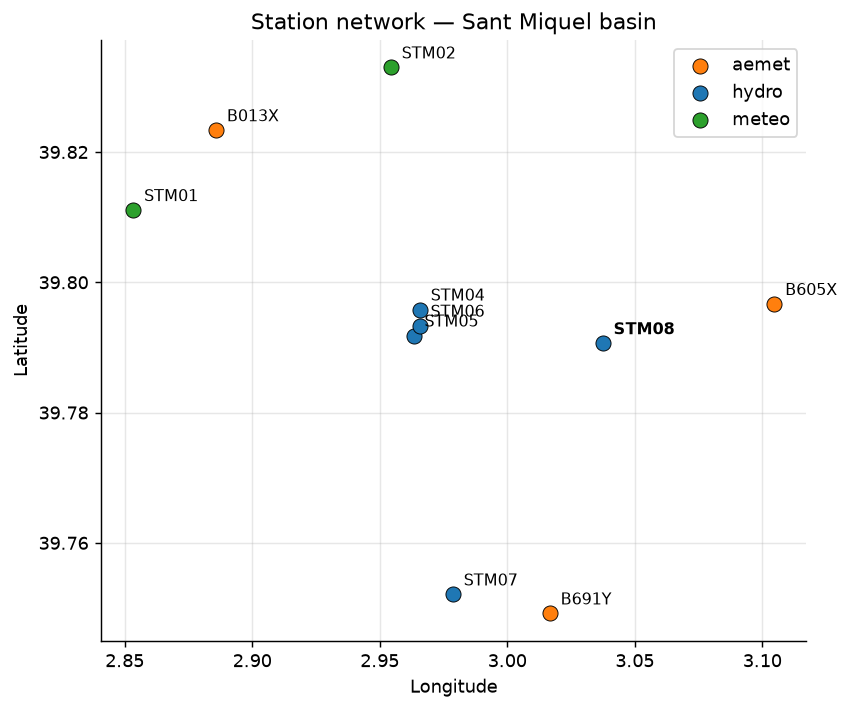
\includegraphics[width=\columnwidth]{station_map.png}
    \caption{Monitoring network used in the current dataset. STM08 is the
    target station at the basin outlet.}
    \label{fig:stations}
\end{figure}

\subsection{Sources and common time window}

Historical STM observations are supplied in Excel files, while the AEMET
series combine UIB-Estrany historical records with production-database
exports. The hydro-station extension is supplied as station-specific
production-database CSV files. The database field named \texttt{WaterLevel}
is expressed in centimetres; the extension loader converts it to metres
before it is written to the common \texttt{HEIGHT\_m} schema. The conversion
is verified against overlapping observations at identical timestamps.

The common modelling window is 2014-09-26 to 2026-07-02. The final date is set
by the AEMET series, although some STM and database files continue to
2026-08-05. All timestamps are treated as UTC. The resulting uniform grid has
618\,769 timestamps, corresponding to approximately 11.8 years at 10-minute
resolution.

\subsection{Data quality and preprocessing}

\subsubsection{Timestamp alignment and resampling}

The STM loggers contain sub-minute timestamp offsets that drift over time.
Before resampling, timestamps are rounded to the nearest minute and duplicate
timestamps are deduplicated. This step is essential: using exact-minute
frequency alignment previously discarded true observations and replaced flood
peaks with interpolated values. At STM08, correcting this issue restored the
historical maximum from 1.31~m to 2.83~m and the corresponding discharge from
19.81 to 87.84~m$^{3}$\,s$^{-1}$.

Instantaneous variables (level and temperature) are handled as follows:
5-minute records are averaged into 10-minute windows, 15-minute records are
linearly interpolated with a three-hour gap cap, and already 10-minute
records are directly aligned. Precipitation is treated as an accumulation:
the source increments are converted into a cumulative curve, interpolated to
the target grid, and differentiated back. This conserves rainfall mass.
Hourly AEMET rainfall is disaggregated using contemporaneous STM01/STM02
10-minute templates, with cumulative interpolation as a conservative
fallback.

\subsubsection{Quality flags and variable selection}

The quality vocabulary is: 0 (good), 1 (suspicious), 2 (wrong), and empty
(not supplied for historical Excel records). Production-database hydro
records with quality 2 are discarded at ingestion. Quality-1 records are
retained, but are explicitly audited. The extension contains 51\,336
quality-1 STM03 records and 6\,888 quality-1 STM05 records. Their transitions
to neighbouring quality-0 data have maximum level changes of 3~mm and 35~mm,
respectively, so no discontinuity-based exclusion is applied.

Water temperature remains in the clean files, grid, and measurements table,
but is excluded from the training table. STM08 water temperature is absent
for 2016--2023 and the validation split has near-complete outages for some
water-temperature stations. Similarly, STM02 air temperature is excluded
because it is weakly seasonal and absent throughout validation. These
decisions avoid training-to-test availability shifts.

Short gaps of up to 24 hours are interpolated. Longer gaps remain NaN and are
paired with a missingness indicator. The final imputation pass fills 21\,156
cells. Discharge is not imputed because a missing discharge value can mean
that the level is outside the rating-curve domain rather than that the sensor
failed.

\subsubsection{Extension harmonization}

After centimetre-to-metre conversion and quality filtering, the extension is
processed using absolute bounds $[-0.5,5.0]$~m, a maximum change of 0.5~m per
10-minute step, and a minimum valid block of 24 hours with at least 70\% valid
values. Only 32 non-null values are removed by these safeguards
after the unit correction.

The extension also exhibits a station-dependent daily oscillation. The
correction procedure is applied uniformly to all six hydro stations. For
quiet rows ($H<0.10$~m), an hour-of-day climatology in the DB-only segment is
compared with a historical climatology restricted to the same calendar
months. The centred difference is subtracted from the DB-only series only
when its amplitude is at least 5~mm and the DB-only range is at least five
times the historical range. This preserves a station's established diurnal
cycle while removing an anomalous thermal-drift component. Corrected source
rows are marked as \texttt{DATA\_TYPE = corrected} in the clean CSVs.

\begin{table}[!t]
    \caption{Hydrological DB extension after unit and quality corrections. The
    final column is the number surviving all harmonization safeguards.}
    \label{tab:extension_quality}
    \centering
    \scriptsize
    \begin{tabular}{@{}lrrrr@{}}
        \toprule
        \textbf{Station} & \textbf{Ext. rows} & \textbf{Non-null} &
        \textbf{After} & \textbf{Diurnal correction} \\
        \midrule
        STM03 & 102\,604 & 48\,531 & 48\,528 & no \\
        STM04 & 82\,759 & 82\,759 & 82\,758 & yes \\
        STM05 & 72\,424 & 57\,643 & 57\,616 & yes \\
        STM06 & 83\,737 & 83\,737 & 83\,736 & no \\
        STM07 & 42\,292 & 42\,292 & 42\,292 & yes \\
        STM08 & 46\,066 & 46\,066 & 46\,066 & yes \\
        \midrule
        \textbf{Total} & 429\,882 & 361\,028 & 360\,996 & \\
        \bottomrule
    \end{tabular}
\end{table}

The diurnal criterion is not triggered for STM03 or STM06. STM03 has a
substantial cycle that is similar to its historical behaviour and is therefore
not removed. STM04 and STM05 meet the criterion under the quiet-row,
season-matched calculation. The source-level correction is retained for
traceability; the grid's per-variable provenance labels identify re-gridded,
derived, and imputed values, while the original correction remains available
in the clean CSVs.

\begin{figure*}[!t]
    \centering
    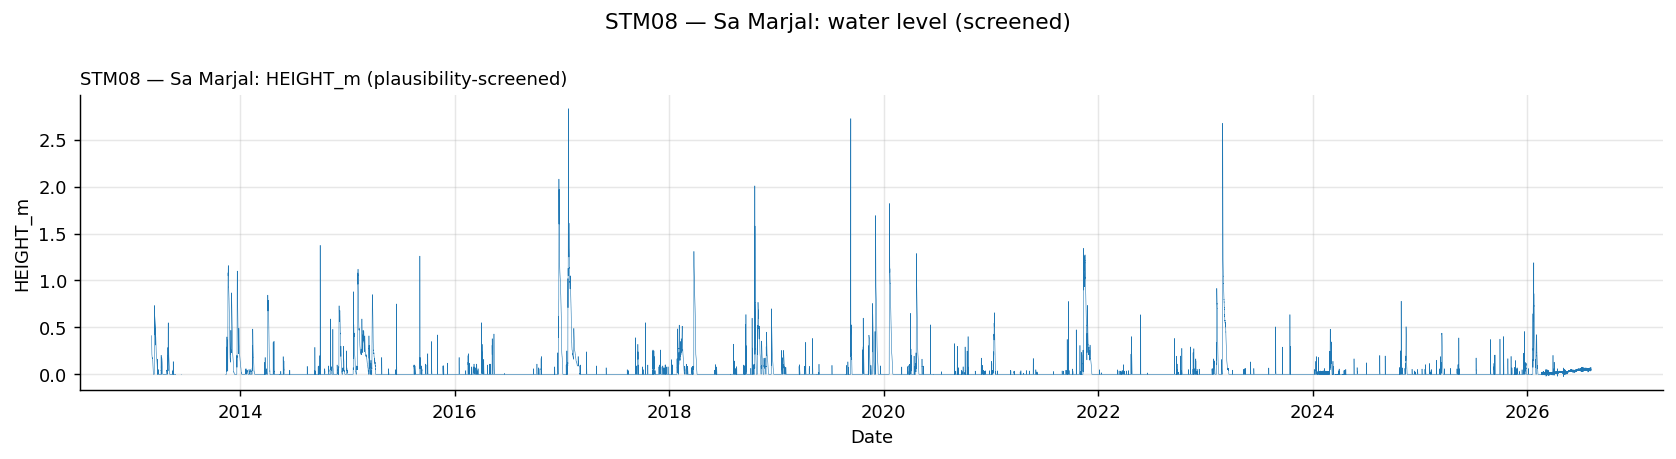
\includegraphics[width=\textwidth]{stm08_overview.png}
    \caption{Screened STM08 water-level record used by the current pipeline.
    The series is highly intermittent, with isolated flood peaks separated by
    long near-zero periods.}
    \label{fig:stm08}
\end{figure*}

\section{Dataset Construction\label{sec:dataset}}

\subsection{Wide grid and measurements table}

The base grid contains 61 columns: 19 measured variables (level, water
temperature, air temperature, and precipitation), six discharge series
derived from rating curves, quality flags, and provenance columns. The
imputed grid contains 80 columns after adding missingness indicators. The
long-format advisor table, \texttt{measurements.parquet}, contains
15\,469\,225 rows and six columns: timestamp, station, variable, value,
quality, and data type. Its data-type counts are 9\,883\,004 observed,
5\,565\,065 derived, and 21\,156 imputed records.

The confirmed drainage topology is:

\begin{equation*}
\begin{gathered}
\mathrm{STM03}\longrightarrow\mathrm{STM04}\longrightarrow\mathrm{STM06}
\longrightarrow\mathrm{STM08},\\
\mathrm{STM05}\longrightarrow\mathrm{STM06},\qquad
\mathrm{STM07}\longrightarrow\mathrm{STM08}.
\end{gathered}
\end{equation*}

Therefore, the engineered total inflow to STM08 is
$Q_{\mathrm{IN}}=Q_{06}+Q_{07}$, rather than the earlier sum of all five
upstream stations. Two lateral-inflow features are also retained:
$\Delta Q_{03,04}=Q_{04}-Q_{03}$ and
$\Delta Q_{05,06}=Q_{06}-Q_{04}-Q_{05}$.

\subsection{Predictors, targets, and splits}

The training table contains 614\,201 rows and 289 columns, including 255
predictors, three future targets, the chronological split, and event labels.
Predictor lags are generated at 1, 2, 3, 6, 12, and 24 hours for the six
hydrological levels, STM01 air temperature, the five precipitation stations,
and upstream discharge. Cumulative precipitation is computed over 3, 6, 12,
24, and 48 hours. The table also contains temporal sine/cosine encodings,
individual upstream-discharge lags, lateral inflows, and total inflow to
STM08. Water temperature and STM02 air temperature are not included as
predictors for the availability reasons described above.

The target columns are the STM08 level at 1, 6, and 24 hours ahead, equivalent
to 6, 36, and 144 ten-minute steps. The split is strictly chronological:

\begin{table}[!t]
    \caption{Chronological supervised-learning split.}
    \label{tab:splits}
    \centering
    \scriptsize
    \begin{tabular}{@{}llll@{}}
        \toprule
        \textbf{Split} & \textbf{Period} & \textbf{Rows} & \textbf{Share} \\
        \midrule
        Train & Sep. 2014--Dec. 2020 & 325\,049 & 52.9\% \\
        Validation & Jan. 2021--Jun. 2022 & 78\,624 & 12.8\% \\
        Test & Jul. 2022--Jul. 2026 & 210\,528 & 34.3\% \\
        \bottomrule
    \end{tabular}
\end{table}

Figure~\ref{fig:ccf} illustrates the exploratory hydrological relationship
that motivated the inclusion of upstream levels and flows. STM04 and STM06
are the strongest level predictors of STM08 in the historical cross-correlation
analysis, with approximate lags of 30 and 60 minutes respectively.

\begin{figure}[!t]
    \centering
    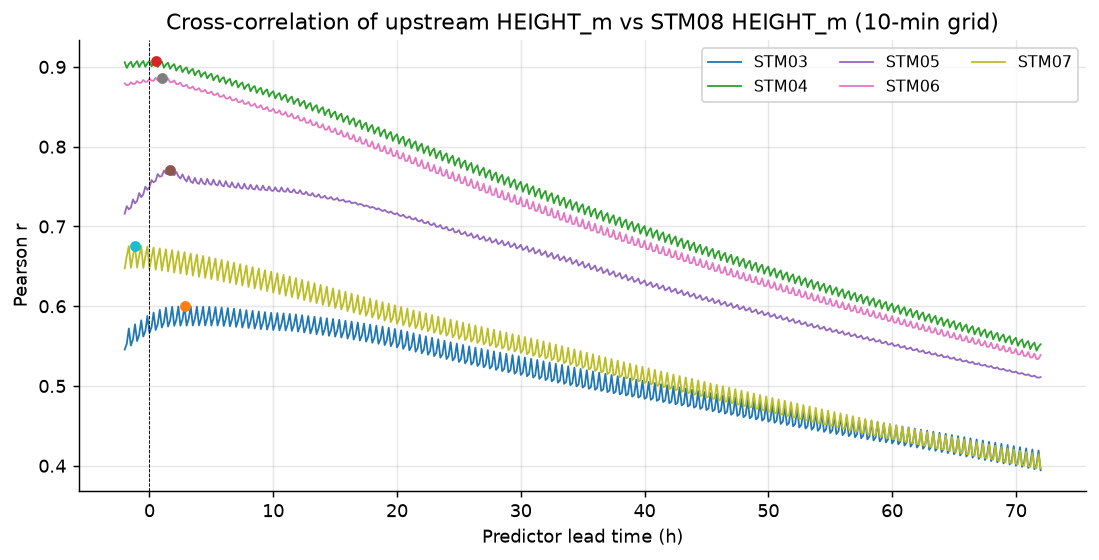
\includegraphics[width=\columnwidth]{ccf_hydro_vs_stm08.png}
    \caption{Historical cross-correlation between upstream hydrological levels
    and STM08. The strongest relationships occur at short routing lags.}
    \label{fig:ccf}
\end{figure}

\section{Flood Event Definition\label{sec:events}}

Flood events are detected on the STM08 discharge series using a peak-over-
threshold procedure with an independence criterion~\cite{Claps2003,Burn2016}.
The event core begins when $Q>0.2$~m$^{3}$\,s$^{-1}$. Consecutive cores with
gaps of up to three hours are grouped, and groups separated by less than six
hours are merged. Boundaries are expanded using $Q>0.05$~m$^{3}$\,s$^{-1}$,
with up to 12 hours of lookback and 24 hours of lookahead. Cores are capped at
72 hours.

As a final global validity criterion, an event must have
$H_{\mathrm{peak}}\geq 0.10$~m. This criterion is applied to all years and
data sources, not only to the database extension. It removes minor pulses and
the residual small oscillations associated with the DB-only sensor drift.

The final catalogue contains 175 valid events: 102 in training, 16 in
validation, and 57 in test. The mean duration is 34.9 hours, the median is
20.0 hours, and the maximum is 108 hours. The largest event reaches
87.84~m$^{3}$\,s$^{-1}$ and 2.83~m at STM08, during January 2017. Seventeen
valid events have peak timestamps after the July 2025 extension boundary.
Each event is assigned to one split using its peak timestamp; the event ID is
then carried into the training table for per-event evaluation.

\section{Data-Driven Baselines\label{sec:baselines}}

\subsection{Models}

Six baseline models are evaluated for each of the three horizons.

\begin{itemize}
    \item \textbf{Persistence:} the current STM08 level is used as the future
    level, $\hat{H}(t+h)=H(t)$.
    \item \textbf{Ridge:} regularised linear regression using the engineered
    predictors. Missing predictors are median-imputed using statistics fitted
    on the training split, and missingness indicators are retained.
    \item \textbf{Random forest:} 100-tree regression ensemble, using the
    training subsample that preserves event rows. The current implementation
    passes missing values natively.
    \item \textbf{XGBoost:} histogram-based gradient boosting with 300 trees,
    learning rate 0.1, maximum depth 8, and native missing-value handling.
    \item \textbf{ARIMA:} univariate STM08 model with order $(2,1,1)$ and
    three Fourier sine/cosine pairs representing the 24-hour cycle.
    \item \textbf{ARIMAX:} the same ARIMA specification with seven curated
    hydrological and rainfall exogenous variables. Future exogenous values
    are not observed during forecasting: they are carried forward from the
    forecast origin, avoiding temporal leakage.
\end{itemize}

The ARIMA order is selected by AIC between $(2,1,1)$ and $(1,1,1)$ on the
last two years of the training split; $(2,1,1)$ is selected. ARIMA and ARIMAX
are fitted on the training split and evaluated using daily rolling origins.
At each origin, a 60-day observed window is used to update the state and a
288-step forecast covers all target leads within the following two days. This
provides row-aligned predictions without using future observations.

\subsection{Metrics}

The primary metric is Nash--Sutcliffe Efficiency (NSE); values near one are
best, while values below zero indicate performance worse than the observed
mean. Kling--Gupta Efficiency (KGE), RMSE, MAE, and PBIAS complement NSE.
Peak magnitude and timing errors and exceedance metrics (POD, FAR, and CSI)
are also calculated at 0.5 and 1.0~m. Results are reported for the complete
test split, its pre-extension validated portion, and the DB-extension
portion. Per-event metrics are computed over the 57 test events.

\subsection{Results}

Table~\ref{tab:test_nse} reports NSE. The test split includes the validated
historical period and the corrected extension. The extension no longer
produces the negative NSE collapse observed before the centimetre conversion.

\begin{table*}[!t]
    \caption{Test NSE by model and horizon. Each cell contains full test /
    validated portion / extension portion.}
    \label{tab:test_nse}
    \centering
    \scriptsize
    \setlength{\tabcolsep}{3pt}
    \begin{tabular}{@{}lccc@{}}
        \toprule
        \textbf{Model} & \textbf{t+1 h} & \textbf{t+6 h} & \textbf{t+24 h} \\
        \midrule
        Persistence & 0.988 / 0.990 / 0.979 & 0.913 / 0.915 / 0.900 &
        0.563 / 0.536 / 0.707 \\
        Ridge & 0.987 / 0.989 / 0.977 & 0.876 / 0.871 / 0.900 &
        0.472 / 0.427 / 0.712 \\
        Random forest & 0.982 / 0.984 / 0.973 & 0.761 / 0.753 / 0.802 &
        0.292 / 0.301 / 0.241 \\
        XGBoost & 0.972 / 0.973 / 0.964 & 0.721 / 0.694 / 0.866 &
        0.091 / 0.017 / 0.486 \\
        ARIMA & 0.856 / 0.852 / 0.875 & 0.777 / 0.764 / 0.845 &
        0.455 / 0.417 / 0.653 \\
        ARIMAX & 0.855 / 0.852 / 0.874 & 0.776 / 0.763 / 0.846 &
        0.454 / 0.417 / 0.654 \\
        \bottomrule
    \end{tabular}
\end{table*}

Persistence is the strongest model by aggregate NSE at all three horizons.
This is expected in an intermittent system: the level changes slowly during
the dominant dry-state portion of the record. Ridge is the strongest
non-persistence model by aggregate NSE, but its positive PBIAS increases with
lead time. At 24 hours, full-test PBIAS is 70.3\% for ridge, 116.2\% for the
random forest, and 138.7\% for XGBoost. The tree models fit the training data
very closely but generalise poorly at long horizons, indicating overfitting
to the intermittent regime and the observed predictor distribution.

ARIMA and leakage-free ARIMAX have nearly identical results. The exogenous
variables do not add measurable aggregate skill when their future values are
not supplied unrealistically. ARIMAX has lower long-horizon bias than the
supervised tree models, but it does not exceed persistence or ridge in NSE.

\begin{table}[!t]
    \caption{Median per-event NSE on the 57 test events.}
    \label{tab:event_nse}
    \centering
    \scriptsize
    \begin{tabular}{@{}lrrr@{}}
        \toprule
        \textbf{Model} & \textbf{1 h} & \textbf{6 h} & \textbf{24 h} \\
        \midrule
        Persistence & 0.184 & $-$1.183 & $-$2.305 \\
        Ridge & 0.363 & $-$1.962 & $-$2.987 \\
        Random forest & 0.297 & $-$5.482 & $-$14.533 \\
        XGBoost & 0.314 & $-$5.927 & $-$10.876 \\
        ARIMA & $-$1.221 & $-$0.731 & $-$2.606 \\
        ARIMAX & $-$1.221 & $-$0.733 & $-$2.511 \\
        \bottomrule
    \end{tabular}
\end{table}

Per-event NSE is substantially lower than aggregate NSE, especially at 6 and
24 hours. This confirms that the rare flood peaks remain the difficult part of
the task even after data-quality corrections. The event table is therefore
more informative for model selection than aggregate scores alone, but its 57
test events still limit statistical certainty.

\begin{figure}[!t]
    \centering
    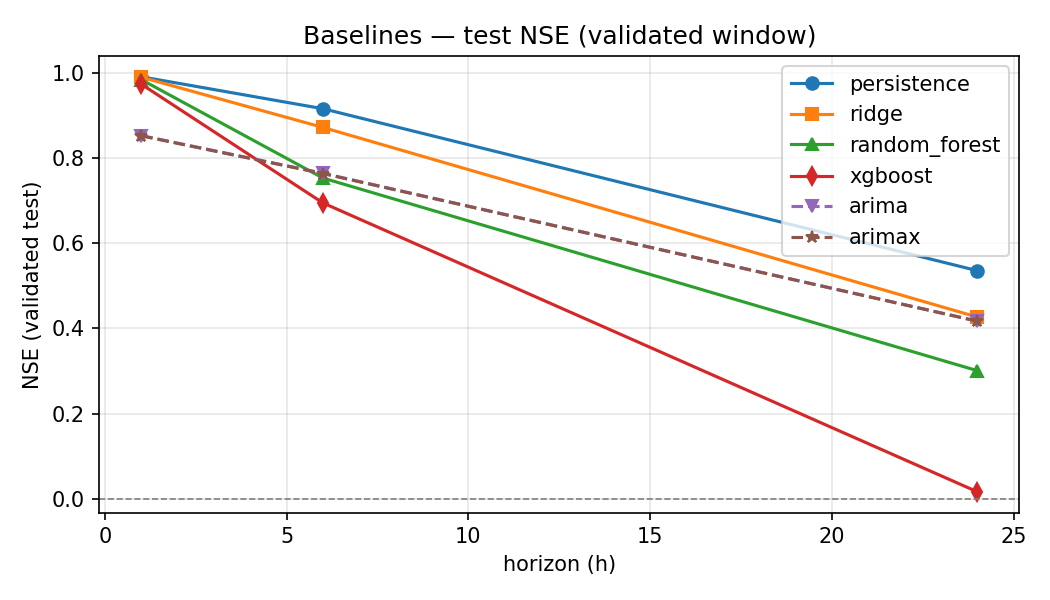
\includegraphics[width=\columnwidth]{baselines_nse.png}
    \caption{Test NSE on the validated portion of the test split. Performance
    decreases with forecast horizon for all baseline families.}
    \label{fig:baseline_nse}
\end{figure}

\section{Physical Model Status and Remaining Scope\label{sec:future}}

The repository contains an initial HEC-HMS project, terrain and basin files,
meteorological configurations, and a Java-based DSS interface. The basin
delineation, parameter calibration, independent event validation, and
uncertainty analysis have not yet been completed. Consequently, there is no
HEC-HMS performance result in the current comparison.

The sequential data-driven phase is also pending. The next modelling stage is
to train multi-horizon LSTM/GRU and Temporal Fusion Transformer models using
the 10-minute training table, the missingness indicators, and the same
chronological splits. Hyperparameter selection must use validation data only.
Subsequent interpretability and comparison phases should include SHAP or an
equivalent feature-attribution method, common event subsets, and a direct
HEC-HMS versus machine-learning comparison.

The current baseline results have four important limitations. First, the
target is highly intermittent, so aggregate NSE is dominated by ordinary
low-flow periods. Second, long predictor gaps remain in the training table;
tree models use native missing values while linear and ARIMA-family models
use train-fitted imputation or carried-forward exogenous values. Third,
quality-1 extension records are retained because their transitions are
continuous, but they remain flagged as suspicious. Fourth, the diurnal drift
correction is a data-quality rule based on historical comparison; it should
be rechecked if new DB data or independent sensor information becomes
available.

\section{Current Conclusions\label{sec:conclusions}}

The current project has reached a reproducible baseline stage. The most
important data finding was that production-database water levels were in
centimetres, while the modelling schema expected metres. Correcting this
conversion restored realistic extension levels and rating-curve discharges.
Quality-2 records were removed, quality-1 records were audited and retained,
and an anomalous DB-only diurnal oscillation was corrected using a
station-comparison rule applied uniformly across the hydro network.

The resulting catalogue contains 175 valid events after applying a global
0.10~m minimum peak-level criterion. Persistence remains the strongest
aggregate baseline, which is an important result rather than a failure: it
quantifies how difficult it is to outperform a state-continuity forecast in a
mostly dry intermittent system. Ridge is the strongest non-persistence model
by aggregate NSE, while ARIMA-family forecasts show comparatively controlled
bias. None of the classical baselines provides consistently strong
event-level performance at 24 hours.

These results establish the reference point for the remaining thesis work.
The next scientific comparison must determine whether HEC-HMS process
representation or sequential neural models can improve flood-event
prediction without sacrificing the robust ordinary-condition behaviour of
the persistence baseline.

\bibliographystyle{abbrv}
\bibliography{bibliography}

\end{document}
